\documentclass[12pt]{article}
\usepackage[a4paper, total={5.5in, 9in}]{geometry}
\usepackage{amsmath}
\usepackage{changepage}
\usepackage[most]{tcolorbox}
\usepackage{textcomp}
\usepackage{tikz}
\usepackage{pgfplots}
\pgfplotsset{compat=1.18}
\usepackage{amsfonts}
\usepackage{graphicx}

\newcommand{\ihat}{\boldsymbol{\hat{\textbf{\i}}}}
\newcommand{\jhat}{\boldsymbol{\hat{\textbf{\j}}}}


\title{Precalculus Worksheet 10.2}
\author{PCL Learning Center}
\date{}

\begin{document}
\maketitle

\begin{center}
    \textit{note: No graphing calculators or electronic devices may be used on this worksheet.}    
\end{center}

\section*{Problem Set 1\\Difficulty level: Normal}
\subsection*{Problem 1}
What are the coordinates of the co-vertices of the hyperbola?
\begin{figure}[!ht]
    \centering
    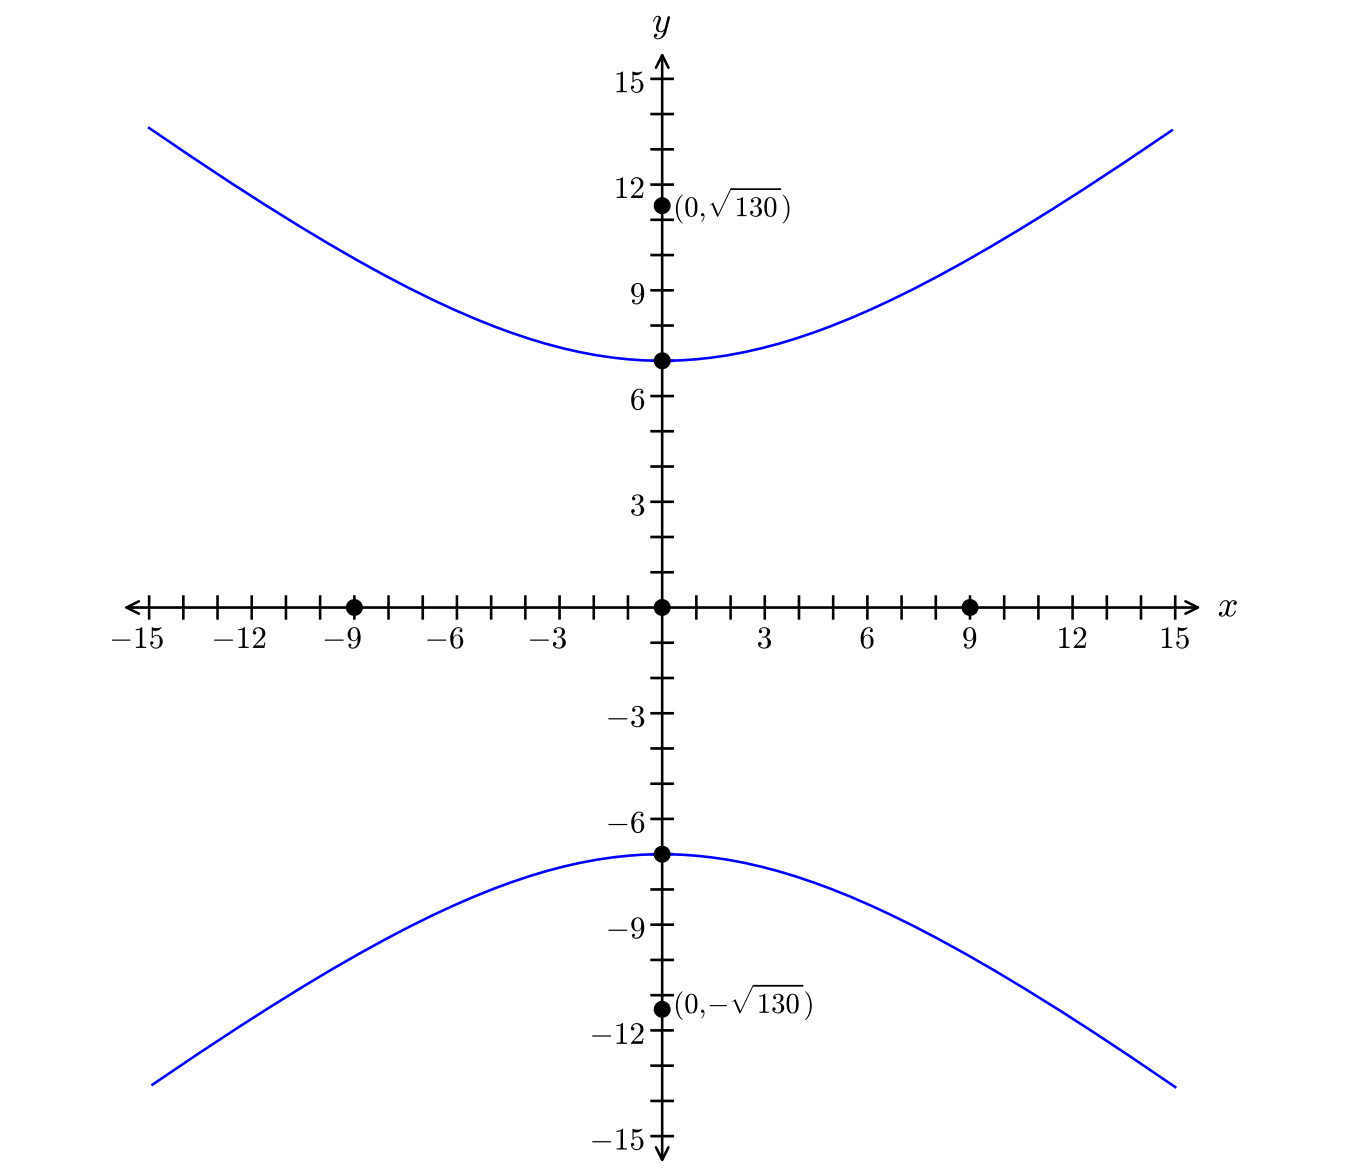
\includegraphics[width=1\linewidth]{1.1.png}
\end{figure}

\newpage
\subsection*{Problem 2}
Identify the coordinates of the co-vertices of the hyperbola shown below.

\begin{figure}[!ht]
    \centering
    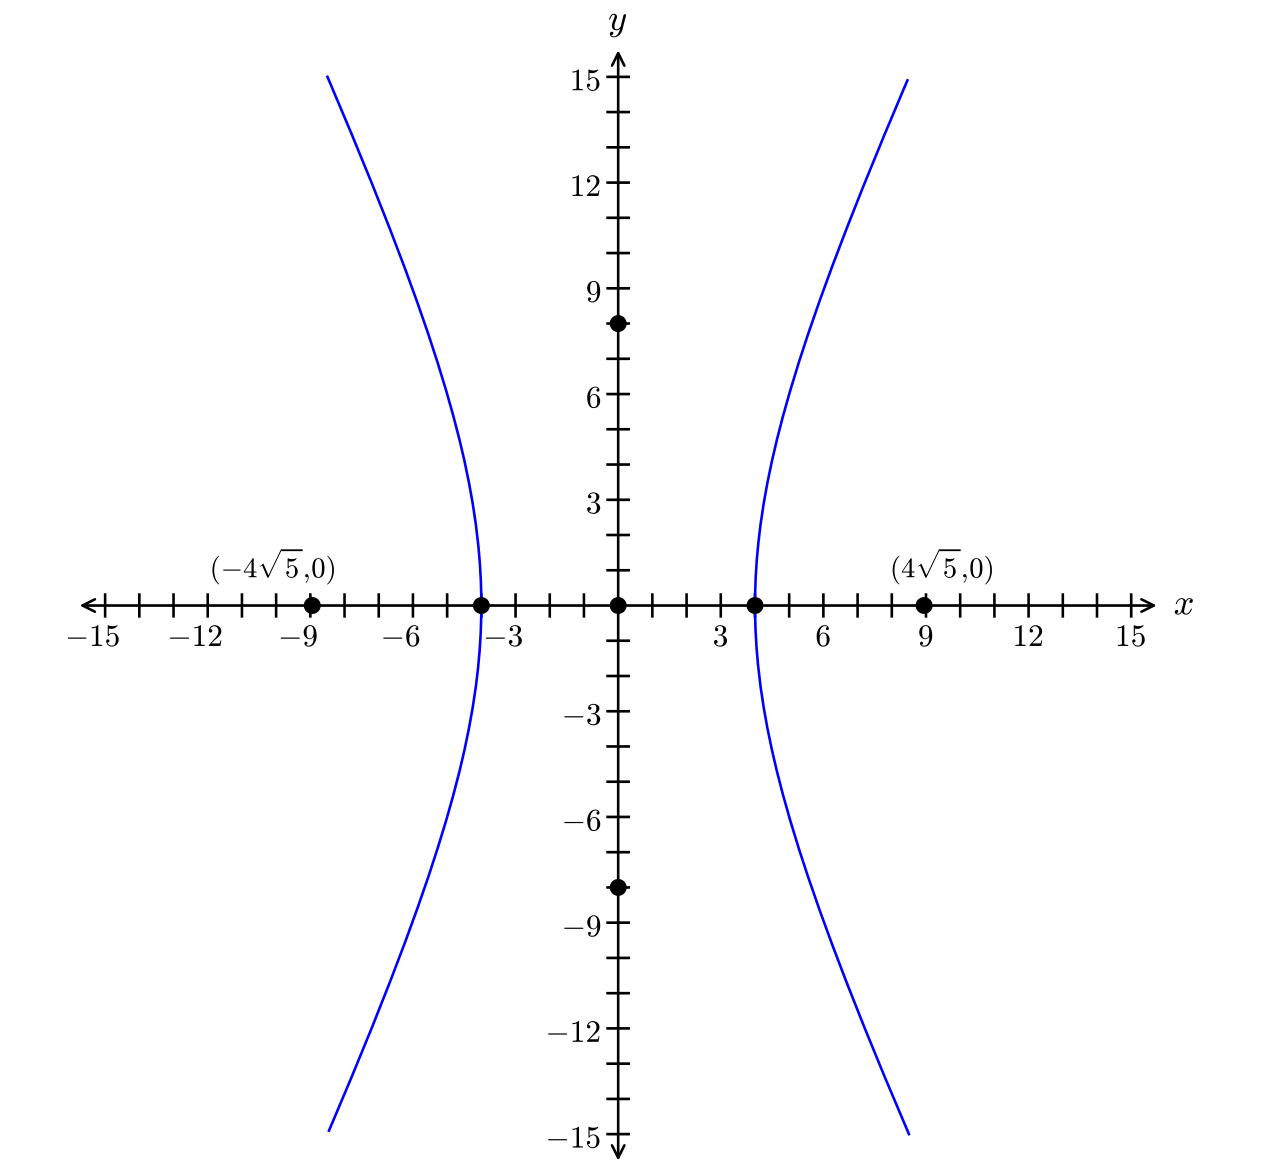
\includegraphics[width=1\linewidth]{6.1.png}
\end{figure}

\subsection*{Problem 3}
What are the asymptotes of the given hyperbola?
\[\dfrac{x^2}{121}-\dfrac{y^2}{81}=1\]

\subsection*{Problem 4}
Find the vertices and foci of the given hyperbola.
\[\dfrac{y^2}{4}-\dfrac{x^2}{25}=1\]

\subsection*{Problem 5}
Write the standard form equation of a hyperbola that has vertices \((0, \pm 1)\) and foci \((0, \pm 5\sqrt{2})\).

\subsection*{Problem 6}
Write an equation for the hyperbola that has vertices \((\pm 7,0)\) and foci \((\pm \sqrt{53},0)\).

\subsection*{Problem 7}
Where must the center of hyperbola be relative to its foci?

\section*{Problem Set 2\\Difficulty level: Hard}
\subsection*{Problem 1}
For the following equations, find the asymptotes for each hyperbola.
\begin{enumerate}
    \item[(a)] \[9x^2-18x-16y^2+32y-151=0\]
    \item[(b)] \[16y^2+96y-4x^2+16x+112=0\]
\end{enumerate}

\newpage
\section*{Solutions for the Set 1}
\subsection*{Problem 1}
\((-9,0)\) and \((9,0)\)
\subsection*{Problem 2}
\((0,-8)\) and \((0,8)\).
\subsection*{Problem 3}
\(y=\pm \dfrac{9}{11}x\)
\subsection*{Problem 4}
The vertices are \((0,\pm 2)\); the foci are \((0, \pm \sqrt{29})\).
\subsection*{Problem 5}
\(y^2-\dfrac{x^2}{49}=1\)
\subsection*{Problem 6}
\(\dfrac{x^2}{49}-\dfrac{y^2}{4}=1\)
\subsection*{Problem 7}
The center of hyperbola must be at the midpoint between its foci.

\section*{Solutions for the Set 2}
\subsection*{Problem 1}
\begin{enumerate}
    \item[(a)] 
    \begin{align*}
    9x^2 - 18x - 16y^2 + 32y - 151 &= 0 \\
    9(x^2 - 2x) - 16(y^2 - 2y) &= 151 \\
    9[(x - 1)^2 - 1] - 16[(y - 1)^2 - 1] &= 151 \\
    9(x - 1)^2 - 9 - 16(y - 1)^2 + 16 &= 151 \\
    9(x - 1)^2 - 16(y - 1)^2 &= 144 \\
    \dfrac{(x - 1)^2}{16} - \dfrac{(y - 1)^2}{9} &= 1 \\
    \text{Asymptotes: } y - 1 &= \pm \dfrac{3}{4}(x - 1)
    \end{align*}

    \item[(b)] 
    \begin{align*}
    16y^2 + 96y - 4x^2 + 16x + 112 &= 0 \\
    16(y^2 + 6y) - 4(x^2 - 4x) &= -112 \\
    16[(y + 3)^2 - 9] - 4[(x - 2)^2 - 4] &= -112 \\
    16(y + 3)^2 - 144 - 4(x - 2)^2 + 16 &= -112 \\
    16(y + 3)^2 - 4(x - 2)^2 &= 16 \\
    \dfrac{(y + 3)^2}{1} - \dfrac{(x - 2)^2}{4} &= 1 \\
    \text{Asymptotes: } y + 3 &= \pm \dfrac{1}{2}(x - 2)
    \end{align*}
\end{enumerate}


\end{document}
